\chapter{Remeshing}
\label{ch:remeshing}

A front-tracking surface is stretched and compressed by the flow; without intervention its
triangles degenerate. Remeshing keeps edge lengths within a window around a target length by
three local operators --- split, collapse and flip --- followed by tangential smoothing, and
optionally restores the enclosed volume that the operators change slightly.

\section{Parameters}

All parameters are in one structure, initialised completely by
\begin{lstlisting}[numbers=none]
void MFTLInitRemeshParams(MFTL_RemeshParameters *params, MFTL_RemeshType type, double target_length,
                          int iterations, MFTL_SmoothMode smooth_mode,
                          double feature_angle_threshold);
\end{lstlisting}
With \texttt{MFTL\_REMESH\_ISOTROPIC} the edge-length window is the Botsch--Kobbelt window
$[\tfrac45 h,\tfrac43 h]$ around the target length $h$. The defaults follow \mftlone: the
Botsch--Kobbelt criterion, the paraboloid vertex fit, quality gates, no volume-conserving
smoothing, load balancing and boundary cleanup on. Important fields:
\begin{description}
  \item[\texttt{criterion}] \texttt{MFTL\_CRITERION\_BOTSCH\_KOBBELT} (edge length),
    \texttt{\_BOTSCH\_KOBBELT\_CURVATURE} (curvature-adaptive length),
    \texttt{\_TRIANGLE\_AREA}, \texttt{\_JIAO};
  \item[\texttt{vertex\_fit}] where a new or moved vertex is placed: \texttt{MFTL\_FIT\_PARABOLOID}
    (least-squares paraboloid through the neighbourhood, LAPACK \texttt{dgelsy}; without LAPACK or
    for a rank-deficient fit the barycentric fit), \texttt{MFTL\_FIT\_BARYCENTRIC},
    \texttt{MFTL\_FIT\_NONE} (the midpoint);
  \item[\texttt{smooth\_mode}, \texttt{max\_smoothing\_iter}] tangential smoothing (vertex- or
    triangle-based centroid, quality-driven, curvature-based);
  \item[\texttt{volume\_conserving\_smoothing}] \texttt{MFTL\_VCSMOOTH\_KUPRAT} or
    \texttt{\_TSUR} after the pass;
  \item[\texttt{load\_balance}, \texttt{boundary\_cleanup}] the parallel driver
    (\S\ref{sec:parallel-remesh});
  \item[\texttt{skip\_*}, \texttt{fixed\_iterations}, \texttt{quiet}, \texttt{mftl1\_criteria}]
    \mftlone-parity switches, all off by default; \multi's front tracking sets them to reproduce
    \mftlone's remeshing;
  \item[\texttt{boundary\_corner\_angle}] the corner threshold of the generalized remesher
    (default $30^\circ$);
  \item[\texttt{stat\_splits}, \texttt{stat\_collapses}, \texttt{stat\_flips},
    \texttt{stat\_recovery\_skipped}] outputs, accumulated by every driver call.
\end{description}

\section{Operators}

\begin{figure}[ht]
\centering
\begin{tikzpicture}[scale=1.05,v/.style={circle,fill=black,inner sep=1.1pt},n/.style={circle,fill=red!70!black,inner sep=1.5pt}]
  % split
  \begin{scope}
    \coordinate (a) at (0,0); \coordinate (b) at (2,0); \coordinate (c) at (1,1.2); \coordinate (d) at (1,-1.2);
    \draw (a)--(b)--(c)--cycle; \draw (a)--(d)--(b);
    \draw[very thick,red!70!black] (a)--(b);
    \foreach \p in {a,b,c,d} \node[v] at (\p) {};
    \node[font=\small] at (1,-1.7) {split};
    \draw[-{Stealth},thick] (2.3,0) -- (2.9,0);
    \begin{scope}[xshift=3.2cm]
      \coordinate (a) at (0,0); \coordinate (b) at (2,0); \coordinate (c) at (1,1.2); \coordinate (d) at (1,-1.2); \coordinate (m) at (1,0.05);
      \draw (a)--(b)--(c)--cycle; \draw (a)--(d)--(b); \draw[red!70!black] (c)--(m)--(d);
      \foreach \p in {a,b,c,d} \node[v] at (\p) {}; \node[n] at (m) {};
    \end{scope}
  \end{scope}
  % collapse
  \begin{scope}[xshift=7cm]
    \coordinate (a) at (0.6,0); \coordinate (b) at (1.4,0); \coordinate (c) at (1,1.2); \coordinate (d) at (1,-1.2);
    \coordinate (e) at (-0.3,0.8); \coordinate (f) at (-0.3,-0.8); \coordinate (g) at (2.3,0.8); \coordinate (h) at (2.3,-0.8);
    \draw (a)--(b)--(c)--cycle; \draw (a)--(d)--(b); \draw (e)--(a)--(f); \draw (e)--(c); \draw (f)--(d); \draw (g)--(b)--(h); \draw (g)--(c); \draw (h)--(d);
    \draw[very thick,red!70!black] (a)--(b);
    \foreach \p in {a,b,c,d,e,f,g,h} \node[v] at (\p) {};
    \node[font=\small] at (1,-1.7) {collapse};
    \draw[-{Stealth},thick] (2.5,0) -- (3.1,0);
    \begin{scope}[xshift=3.6cm]
      \coordinate (m) at (1,0); \coordinate (c) at (1,1.2); \coordinate (d) at (1,-1.2);
      \coordinate (e) at (-0.3,0.8); \coordinate (f) at (-0.3,-0.8); \coordinate (g) at (2.3,0.8); \coordinate (h) at (2.3,-0.8);
      \draw (e)--(m)--(f); \draw (g)--(m)--(h); \draw (c)--(m)--(d); \draw (e)--(c)--(g); \draw (f)--(d)--(h);
      \foreach \p in {c,d,e,f,g,h} \node[v] at (\p) {}; \node[n] at (m) {};
    \end{scope}
  \end{scope}
\end{tikzpicture}\\[2ex]
\begin{tikzpicture}[scale=1.05,v/.style={circle,fill=black,inner sep=1.1pt}]
  \coordinate (a) at (0,0); \coordinate (b) at (2.2,0); \coordinate (c) at (1.1,1.0); \coordinate (d) at (1.1,-1.0);
  \draw (a)--(c)--(b)--(d)--cycle; \draw[very thick,red!70!black] (a)--(b);
  \foreach \p in {a,b,c,d} \node[v] at (\p) {};
  \draw[-{Stealth},thick] (2.5,0) -- (3.1,0);
  \begin{scope}[xshift=3.4cm]
    \coordinate (a) at (0,0); \coordinate (b) at (2.2,0); \coordinate (c) at (1.1,1.0); \coordinate (d) at (1.1,-1.0);
    \draw (a)--(c)--(b)--(d)--cycle; \draw[very thick,red!70!black] (c)--(d);
    \foreach \p in {a,b,c,d} \node[v] at (\p) {};
  \end{scope}
  \node[font=\small] at (2.8,-1.5) {flip};
\end{tikzpicture}
\caption{The three topological operators. Split inserts a vertex on a long edge and splits both
adjacent triangles; collapse merges the two ends of a short edge into one vertex (removing two
triangles); flip replaces the diagonal of two triangles.}
\label{fig:operators}
\end{figure}

The operators (\texttt{mftl\_remeshing.h}) act rank-locally on stored entities
(Figure~\ref{fig:operators}):
\begin{description}
  \item[\fn{MFTLSplitEdge}] splits an edge at its midpoint (an interior or a boundary edge,
    never a REMOTE one) and returns the new vertex; the new vertex is placed by the displacement
    rule (\S\ref{sec:displacement}). \fn{MFTLSplitEdgeWithFit} then moves it onto the fitted
    surface.
  \item[\fn{MFTLCollapseEdge}] collapses $a\to b$; the survivor moves to the midpoint (or the
    fitted point with \fn{MFTLCollapseEdgeWithFit}).
  \item[\fn{MFTLFlipEdge}] flips an interior edge in place.
\end{description}
Removed entities are flagged \texttt{MFTL\_FLAG\_DEAD} during a pass;
\fn{MFTLFinalizeRemeshing} compacts the arrays afterwards (before any redistribution). The
approval gates \fn{MFTLSplitApproved}, \fn{CollapseApproved} and \fn{FlipApprovedWithParams}
apply the criterion, the link condition, quality and dihedral-angle gates, and the protection
of sharp features (\fn{MFTLDetectFeatures} flags edges whose dihedral angle exceeds the feature
angle). The operators keep the twin states: splits create LOCAL pairs and a boundary split
gives both halves the parent's tag; a collapse merges the states of the two outer
half-edges and is refused if one of them is REMOTE.

\paragraph{Criteria.} The Botsch--Kobbelt criterion splits edges longer than
\texttt{max\_edge\_length} and collapses edges shorter than \texttt{min\_edge\_length}. Its
curvature variant replaces the fixed target by the edge length that keeps the deviation from
the surface below $\varepsilon$ (\fn{MFTLBotschKobbeltCurvatureThreshold}): with
$\kappa_{\max}=\bar H+\sqrt{\bar H^2-\bar K}$ per endpoint, $\bar H$ and $\bar K$ being the stored
mean and Gaussian curvatures (Chapter~\ref{ch:geometry}),
\begin{equation}
  L = \sqrt{6\varepsilon/\kappa_{\max}-3\varepsilon^2},
\end{equation}
clamped to the window; the edge is split above $\tfrac43L$ and collapsed below $0.8L$. The
triangle quality used by the gates is the \mftlone{} measure
$q=(\text{perimeter}^2/A)/20.78460969$ (1 for an equilateral triangle, larger is worse;
\fn{MFTL\_TriangleQuality}).

\section{Smoothing and volume conservation}
\label{sec:volume-recovery}

\fn{MFTLSmoothTangential} (and \fn{MFTLSmoothTangentialWithParams}) move interior vertices in
their tangent plane towards the centroid of their neighbours or fan; vertices on a feature line
move along it; corners and boundary or rim vertices stay fixed. Two volume-conserving smoothers
are available: Kuprat's volume-conserving Laplacian (\fn{MFTLVolumeConservingSmoothing}, per edge
an exact first-order volume correction) and Jiao's TSUR3D null-space smoothing
(\fn{MFTLTSUR3D}); \fn{MFTLRoughnessSmoothing} applies them where the roughness exceeds its
thresholds. The serial versions refuse to run on a distributed mesh; the \texttt{...Parallel}
versions gate every edge to ``both endpoints owned, complete local fan''.

\paragraph{Volume recovery} (\fn{MFTLVolumeRecovery}\texttt{(obj, V\_target)}, collective) moves every
owned vertex along its normal by
\begin{equation}
  h = \frac{V-V_{\text{target}}}{A_{\text{eff}}}
\end{equation}
where $A_{\text{eff}}$ weights each owned triangle by the fraction of its corners owned by the rank
(exact first order in parallel); after the first step the slope is replaced by the measured
secant. It iterates until the relative error is below $10^{-12}$ (at most 10 steps; the stop
decision is reduced over ranks) and returns the final relative error. For a body that does not
enclose a volume by itself (open or wrapping) it does nothing and returns 0; use
\fn{MFTLPhaseSetVolumeRecovery} for sets.

\section{Surfaces with boundary: the generalized remesher}

Open bodies --- and closed bodies opted in with
\fn{MFTLObjectSetRemeshMode}\texttt{(obj, MFTL\_REMESH\_MODE\_GENERALIZED)} --- are remeshed by the
generalized, boundary-aware remesher. Closed bodies in the default mode use the closed-surface
remesher (with \texttt{mftl1\_criteria} set: bit-for-bit the \mftlone{} criteria). The selection
depends only on the declared class and the explicit mode, never on periodicity or on a body
touching a seam.

\paragraph{Link condition.} A collapse must not change the topology. The generalized remesher
uses the link condition on the complex augmented by one virtual vertex $\omega$ joined to every
boundary vertex (a virtual triangle $(u,v,\omega)$ per boundary edge): the collapse of $ab$ is
legal iff $\operatorname{Lk}(a)\cap\operatorname{Lk}(b)=\operatorname{Lk}(ab)$ in the augmented
complex. This single test forbids pinching a narrow strip, merging two boundary loops, creating
bow-ties, closing small holes and letting components vanish, while allowing the collapse of an
``ear'' triangle at the boundary.

\paragraph{Boundary curves and corners.} Every boundary tag has a boundary-curve mode
(\fn{MFTLObjectSetBoundaryCurve}):
\begin{itemize}
  \item \texttt{MFTL\_BCURVE\_REPRESENTED} (default): the curve is the interpolating Catmull--Rom
    spline through the loop's vertices; new boundary vertices are placed on it, so repeated
    remeshing does not shrink the loop;
  \item \texttt{MFTL\_BCURVE\_CONSTRAINED}: new and moved boundary vertices are projected by an
    application callback \texttt{MFTL\_BoundaryProjector} (a wall line, a ring, a support);
    \texttt{freeze} keeps the boundary vertices of the tag fixed during smoothing (used for
    pinned boundaries).
\end{itemize}
A boundary vertex whose turning angle exceeds the corner angle, or that carries
\texttt{MFTL\_VFLAG\_CORNER}, is a corner: it is never moved, merged or collapsed.

\paragraph{Other rules.} Boundary edges are never flipped; flips next to the boundary aim at
valence 6 inside, 4 on a straight boundary and $\operatorname{round}(\theta/60^\circ)+1$ at a
boundary vertex with interior angle $\theta$. Boundary vertices move only along their boundary
curve during smoothing. The volume-conserving smoothers act only on edges whose endpoints both
have closed fans.

\paragraph{Class-guarded volume recovery.} The drivers recover a body's volume only when it is
defined: its own volume for a closed compact body, the volume of its singleton phase set when
that is \texttt{MFTL\_DEFINED}, and nothing otherwise (counted in
\texttt{stat\_recovery\_skipped}).

\section{Drivers}
\label{sec:serial-bracket}

\paragraph{Serial.} \fn{MFTLRemeshEnsemble}\texttt{(ens, params)} runs the split, collapse, flip and
smoothing passes on every object, compacts, applies the optional volume-conserving smoothing and
the class-guarded volume recovery. Its edge kernel is rank-local, so on a distributed ensemble it
is run inside a \emph{serial bracket}:
\begin{lstlisting}[numbers=none]
MFTL_SerialBracket br;
MFTLEnsembleBeginSerial(ens, &br);      /* gather every object on rank 0 */
MFTLRemeshEnsemble(ens, &params);
MFTLEnsembleEndSerial(ens, &br, 1);     /* restore the decomposition and redistribute */
\end{lstlisting}
The bracket is also the way to run any serial kernel (TSUR3D, restart output) on a distributed
ensemble.

\paragraph{Parallel.}
\label{sec:parallel-remesh}
\fn{MFTLRemeshEnsembleParallel}\texttt{(ens, params)} (collective) chooses the algorithm:
\begin{itemize}
  \item on one rank, the serial kernel;
  \item for an ensemble of type \texttt{MFTL\_ENSEMBLE\_DISPERSED} whose largest body box is
    smaller than $0.5\,h_{\min}$ ($h_{\min}$: the smallest rank-box width), \emph{centering}:
    the ensemble is gathered on rank 0 and remeshed serially
    (\fn{MFTLRemeshEnsembleDispersedCentering});
  \item otherwise the \mftlone{} \emph{two-pass shift scheme}
    (\fn{MFTLRemeshEnsembleShiftScheme}).
\end{itemize}
The shift scheme (Figure~\ref{fig:shift}) first computes an x-only slab decomposition that
equalises the number of owned triangles per slab (\fn{MFTLRedistributeEnsembleLoadBalanced}); on a
decomposition that is not x-only, a temporary x-only layout is used and the native one restored
afterwards. Pass~1 remeshes on every rank the edges that are interior to it (both endpoints and
the complete fans owned); per-rank blocks of global ids are handed out before any split. Then
the cuts are shifted by $\max(0.2\,w_{\min},3\ell_{\text{ref}})$ ($w_{\min}$: the smallest slab
width, $\ell_{\text{ref}}$: \texttt{reference\_length}; \fn{MFTLShiftOwnershipRanges}) so that the
edges that straddled a cut become interior, and pass~2 remeshes them. Finally the few edges
that straddle both the old and the shifted cut are remeshed after gathering them on rank 0
(boundary cleanup), and a split cleanup pass follows. The mesh is returned redistributed on the
native decomposition, at a quiescent point.

\begin{figure}[ht]
\centering
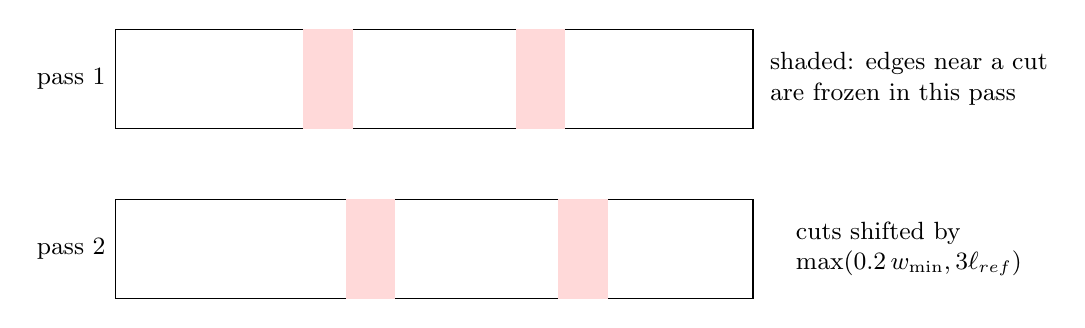
\begin{tikzpicture}[scale=0.9]
  \foreach \y/\lab/\sh in {2.4/pass 1/0, 0/pass 2/0.6} {
    \draw (0,\y) rectangle (9,\y+1.4);
    \foreach \x in {3,6} { \draw[very thick,dashed] (\x+\sh,\y) -- (\x+\sh,\y+1.4); }
    \foreach \x in {3,6} { \fill[red!15] (\x+\sh-0.35,\y) rectangle (\x+\sh+0.35,\y+1.4); }
    \node[left,font=\small] at (0,\y+0.7) {\lab};
  }
  \node[font=\small,align=left] at (11.2,3.1) {shaded: edges near a cut\\ are frozen in this pass};
  \node[font=\small,align=left] at (11.2,0.7) {cuts shifted by\\ $\max(0.2\,w_{\min},3\ell_{\text{ref}})$};
\end{tikzpicture}
\caption{The two-pass shift scheme on x-only slabs: edges near a cut are frozen in pass 1 and
remeshed in pass 2 after the cuts have been shifted.}
\label{fig:shift}
\end{figure}

\fn{MFTLRemeshEnsembleParallel} runs \texttt{MFTL\_ENSEMBLE\_SPANNING} ensembles (large interfaces)
always with the shift scheme. The example of \S\ref{sec:ex-remesh} runs a serial and a parallel
cycle.
